\documentclass[12pt,utf8,notheorems,compress]{beamer}

\usepackage[english]{babel}

\usepackage{mathtools}
\usepackage{ragged2e}
\usepackage{multicol}
\usepackage{tabto}

\usepackage[protrusion=true,expansion=false]{microtype}

\setlength\parskip{\medskipamount}
\setlength\parindent{0pt}

\newcommand{\RR}{\mathbb{R}}
\newcommand{\Set}{\mathrm{Set}}
\newcommand{\defeq}{\vcentcolon=}

\title{Homotopy type theory}
\author[Arbeitsseminar Geometrie/Topologie]{\vspace{-1em}\\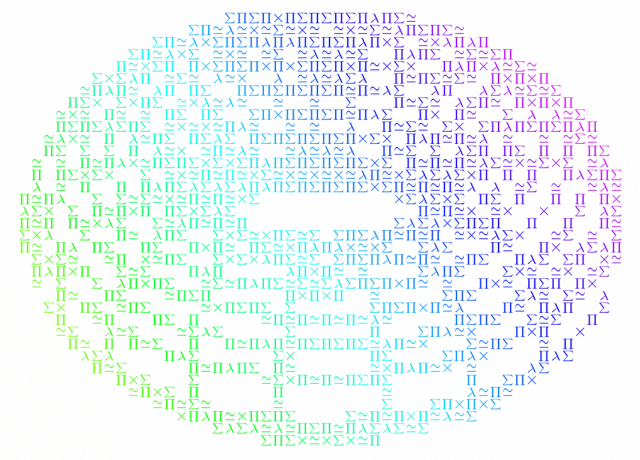
\includegraphics[scale=0.3]{torus.png} \\[0.5em] Ingo Blechschmidt \\[-0.3em] {\scriptsize November 25th, 2014}}
\date{November 25th, 2014}

\usetheme{Warsaw}
\usecolortheme{seahorse}
%\usefonttheme{default}
\usepackage{kurier}
\useinnertheme{rectangles}

\setbeamertemplate{frametitle}[default][colsep=-4bp,rounded=false,shadow=false,center]

\setbeamertemplate{headline}{}
\setbeamertemplate{navigation symbols}{}

\newcommand{\backupstart}{
  \newcounter{framenumberpreappendix}
  \setcounter{framenumberpreappendix}{\value{framenumber}}
}
\newcommand{\backupend}{
  \addtocounter{framenumberpreappendix}{-\value{framenumber}}
  \addtocounter{framenumber}{\value{framenumberpreappendix}} 
}

\newcommand*\oldmacro{}%
\let\oldmacro\insertshorttitle%
\renewcommand*\insertshorttitle{%
  \oldmacro\hfill\insertframenumber\,/\,\inserttotalframenumber\hfill}

\newcommand{\hil}[1]{{\usebeamercolor[fg]{item}{\textbf{#1}}}}

\newcommand{\img}[3]{\begin{center}\includegraphics[scale=#1]{#2}\\#3\end{center}}
%\newcommand{\imageslide}[3]{\frame{\frametitle{#1}\img{#2}{#3}}}

\setbeameroption{show notes}
\setbeamertemplate{note page}[plain]

\begin{document}

\frame{\titlepage}

\frame[t]{\frametitle{Outline}\tableofcontents}

\note{\justifying\fontsize{8pt}{9.6}\selectfont
  \setlength{\columnsep}{1em}
  \begin{multicols}{2}
    Homotopy type theory is a new branch of mathematics that combines
    aspects of several different fields in a surprising way. It is part of
    Voevodsky's \emph{univalent foundations} program and based on a recently
    discovered connection between homotopy theory and type theory, a branch
    of mathematical logic and theoretical computer science.

    In homotopy type theory, any set (really: \emph{type}) behaves like a
    topological space, or more precisely, a homotopy type. The basic notion
    of equality is reimagined in an interesting way: Analogous to how two
    given points in a space may be joined by more than one path, two
    elements of a set can be equal in many ways. A new axiom, the
    \emph{univalence axiom}, posits that equivalent structures really are
    the same, thus formalizing a widespread notational practice.

    Besides explaining how working in homotopy type theory feels like, the
    talk will give answers to the listed questions.
    The talk does not assume any background in formal logic or type theory.
    \columnbreak

    \begin{itemize}
    \justifying
    \item What are logical foundations for mathematics and why should we care?
    \item What are the disadvantages of traditional set-based approaches to foundations?
    \item Why is the development of homotopy theory radically simplified in
    homotopy type theory?
    \item How are the seemingly diverse activities of \emph{proving
    propositions} and \emph{exhibiting constructions} identified?
    \item How do inductive definitions of important spaces concisely capture
    their homotopy-theoretic content?
    \item Why is homotopy type theory a major step towards practically useful
    and easily applicable proof assistants?
    \end{itemize}
  \end{multicols}
}


\section{Foundations}

\subsection{What are foundations?}

\frame[t]{\frametitle{What are foundations?}
  \begin{itemize}
    \item Foundations set the logical context for doing maths.
    \item Their details don't matter in everyday work (mostly).
    \item But their main concepts do.
  \end{itemize}

  \pause
  \begin{itemize}
    \item Classical foundations are \emph{set-based} (ZF, ZFC, \ldots):
          \hil{Everything is a set.}
    \item $0 \defeq \emptyset$, \quad
          $1 \defeq \{0\}$, \quad
          $2 \defeq \{0,1\}$, \quad
          $\ldots$
    \item $(x,y) \defeq \{ \{x\}, \{x,y\} \}$ \quad (Kuratowski pairing)
    \item $(x,y,z) \defeq (x,(y,z))$
    \item maps: $(X,Y,R)$ with $R \subseteq X \times Y$ such that \ldots
  \end{itemize}
}

\note{
  \begin{itemize}
    \item Foundations allow us to be maximally precise.
    \item A \emph{proof} as commonly understood is really a shorthand for a
    (never spelled out) fully formal proof.
    \item Unlike informal proofs, the correctness of a formal proof can be
    checked mechanically.
  \end{itemize}

  \img{0.5}{logicomix}{Logicomix: An Epic Search for Truth}
}


\subsection{What's problematic with set-based foundations?}

\frame[t]{\frametitle{What's wrong with set-based foundations?}
  Set-based foundations \ldots
  \begin{itemize}
    \item allow to formulate nonsensical questions,
    \item do not reflect typed mathematical practice,
    \item require complex encoding of ``higher-level'' subjects,
          complicating interactive proof environments.
  \end{itemize}
}

\note{
  \begin{itemize}
    \item Examples for questions which can be formulated:
    \begin{itemize}
      \item Is $2 = (0,0)$? (No, when using my definitions.)
      \item Is $\sin \in \pi$? (Depends on your definitions.)
    \end{itemize}
    \item\justifying In ordinary practice, these questions would be deemed as nonsensical,
    since they disrespect the \emph{types} of mathematical objects and are not
    invariant under isomorphisms of the involved structures.
  \end{itemize}

  \begin{itemize}
    \item\justifying Fully unravel the definition of ``manifold'' in set-theoretical
    language to get a grasp of the complex encodings needed.
    \item This is no problem for humans, but it is for machines.
  \end{itemize}

  \begin{itemize}
    \item Note: Set theory is perfectly fine for studying \emph{sets}.
  \end{itemize}
}


\section{Basics on homotopy type theory}

\subsection{What is homotopy type theory?}

\frame[t]{\frametitle{What is homotopy type theory?}
  \begin{itemize}
  \end{itemize}
}

\backupstart
\backupend

\end{document}

XXX: Illustration of sets and types
